\section{Thermal diffusion}

This section shows how the thermal diffusion coefficients relate to those in a binary system in the binary limit. The section also gives some insight into different definitions of the thermal diffusion coefficient, with the aim of showing that the definition is not arbitrary if one wishes to relate the ternary coefficients to the respective binary coefficients.

\subsection{Notation}

For fluxes the superscript $(i, j)$ is used, where $i$ is the basis ($m$ for mass-based, $n$ for mole based) and $j$ is the frame of reference. Thermal diffusion coefficients are denoted $D_{T, i}$, the superscript $(z)$ denotes thermal diffusion coefficients as defined by Ortiz de Zárate \cite{ortiz2019definition}, while superscripts $(m)$ and $(n)$ denote the independent thermal diffusion coefficients in the centre of mass, and centre of moles FoR, as defined in ref. \cite{retmie}. 

Similarly, diffusion matrices are superscripted with $(x)$ and $(w)$ to denote those defined by Ortiz de Zárate using the same notation, while superscripts $(m)$ and $(n)$ are used for the independent diffusion matrices in the CoM and CoN FoR as defined in ref. \cite{retmie}.

The notation $D_{T,i}^{(z,tj)}$ denotes the thermal diffusion coefficient of species $i$ in a ternary mixture with species $j$ taken to be the dependent species, as defined in ref. \cite{ortiz2019definition} while $D_{T,i}^{(z,bj)}$ denotes the thermal diffusion coefficient of species $i$ in a binary mixture, with species $j$ taken to be the dependent species.

Boldface roman font ($\Vec{v}$) is used to indicate vectors, and slanted underlined boldface figures ($\Mat{D}$) are used to indicate matrices. The notation $\nabla \Vec{v}$, should be understood not as a dot product, but as a vector of gradients (i.e. $\nabla \Vec{v} \equiv (\nabla v_1, \nabla v_2, ...)^\top$, in which case the equations should be understood to hold componentwise for these gradients.

\subsection{Definitions of the thermal diffusion coefficient}

The default definition of the thermal diffusion coefficient in a multicomponent mixture in the KineticGas package is

\begin{equation}
    J_i^{(n,m)} = D_{T,i}^{(m)} \nabla \ln T - \sum_{j \neq \ell} D_{ij}^{(m)} \nabla c_j
\end{equation}

where the superscript $(n, m)$ indicates that the flux is on a molar basis in the centre of mass (CoM) frame of reference (FoR), and the superscripts $(m)$ indicate that the coefficients apply to the CoM FoR. Component $\ell$ is the dependent component, which defaults to the last component in the mixture. For later convenience, we rewrite this for a ternary system as

\begin{equation}
    \begin{split}
        \begin{pmatrix}J_1^{(n,m)} \\ J_1^{(n,m)} \end{pmatrix} &= - \Mat{D}^{(m)} \begin{pmatrix} \nabla c_1 \\ \nabla c_1 \end{pmatrix} + \begin{pmatrix} D_{T,1}^{(m)} \\ D_{T,2}^{(m)} \end{pmatrix} \nabla \ln T\\
        \Vec{J}^{(n, m)} &= - \Mat{D}^{(m)} \nabla \Vec{c} + \Vec{D}_T^{(m)} \nabla \ln T
    \end{split}
    \label{eq:Dtm_def}
\end{equation}

In the centre of moles frame of reference, the diffusion- and thermal diffusion coefficients are defined by
\begin{equation}
    \begin{split}
        \Vec{J}^{(n, n)} &= - \Mat{D}^{(n)} \nabla \Vec{c} + \Vec{D}_T^{(n)} \nabla \ln T.
    \end{split}
    \label{eq:DTn_def}
\end{equation}
and they are related by
\begin{equation}
    \Mat{D}^{(n)} = \Mat{\Psi}^{n \leftmapsto m} \Mat{D}^{(m)}, \quad \Vec{D}_T^{(n)} = \Mat{\Psi}^{n \leftmapsto m} \Vec{D}_T^{(m)},
\end{equation}
with $\Mat{\Psi}^{n \leftmapsto m}$ being the transformation matrix given in the supporting information of \cite{retmie}, adapted to a $(N_c - 1) \times (N_c - 1)$ matrix, rather than the original $N_c \times N_c$ matrix, by using the linear dependence of the fluxes.

In 2019 Ortiz de Zárate \cite{ortiz2019definition} showed that one can define thermal diffusion coefficients that are equivalent in the centre of mass and centre of moles frames of reference, if one defines them through either

\begin{equation}
    \begin{split}
        \Vec{J}^{(n, n)} &= - c \left( \Mat{D}^{(x)} \nabla \Vec{x} + \Mat{X} \Vec{D}_T^{(z)} \nabla T \right), \quad \text{or}\\
        \Vec{J}^{(m, m)} &= - \rho \left( \Mat{D}^{(w)} \nabla \Vec{w} + \Mat{W} \Vec{D}_T^{(z)} \nabla T \right)
    \end{split}
    \label{eq:zarate_def}
\end{equation}

where the matrices $\Mat{X}$ and $\Mat{W}$ are given by
\begin{equation}
    X_{ij} = \delta_{ij} x_i - x_i x_j, \quad W_{ij} = \delta_{ij} w_i - w_i w_j.
\end{equation}
The superscripts $(x)$ and $(w)$ indicate diffusion matrices that apply in the centre of moles and centre of mass FoR respectively, when using these definitions. The superscript $(z)$ marks the thermal diffusion coefficients as defined by Eq. \eqref{eq:zarate_def}. When using this definition of the thermal diffusion coefficient, Ortiz de Zárate shows that 
\begin{equation}
    \lim_{x_2 \to 0} D_{T,1}^{(z,t3)} = D_{T,1}^{(z,b3)},
\end{equation}
where $D_{T,1}^{(z,t)}$ is the thermal diffusion coefficient of species 1 in a ternary mixture, and $D_{T,1}^{(z,b3)}$ is the thermal diffusion coefficient of species 1 in a binary mixture with species 3, both as defined by Eq. \eqref{eq:zarate_def}.
that is: For a ternary system (1, 2, 3), when the mole fraction of species 2 tends to zero, the thermal diffusion coefficient of species 1 approaches the thermal diffusion coefficient of species 1 in the binary mixture (1, 3). This relation follows from an argument analogous to that in section \ref{sec:diff_indep}.

For an ideal gas can relate the thermal diffusion coefficients $\Vec{D}_T^{(n)}$ to the $\Vec{D}_T^{(z)}$, by rewriting Eq. \eqref{eq:DTn_def} as 
\begin{equation}
    \begin{split}
        \Vec{J}^{(n, n)} &= - \Mat{D}^{(n)} ( c \nabla \Vec{x} + \Vec{x} \nabla c) + \Vec{D}_T^{(n)} \nabla \ln T \\
        &= - \Mat{D}^{(n)} ( c \nabla \Vec{x} - \Vec{x} c \nabla \ln T) + \Vec{D}_T^{(n)} \nabla \ln T \\
        &= - c \Mat{D}^{(n)} \nabla \Vec{x} + \frac{1}{T} \left( \Vec{D}_T^{(n)} + c \Mat{D}^{(n)}\Vec{x}\right) \nabla T
    \end{split}
\end{equation}
such that $\Vec{D}_T^{(z)}$ is given by the solution to
\begin{equation}
    - c \Mat{X} \Vec{D}_T^{(z)} = \frac{1}{T} \left( \Vec{D}_T^{(n)} + c \Mat{D}^{(n)}\Vec{x}\right), \quad \text{Ideal gas}
    \label{eq:DTz_DTn_relate}
\end{equation}
where we have made use of $\nabla c = c \nabla \ln T$ for an ideal gas. For a non-ideal gas the corresponding expression is
\begin{equation}
    \begin{split}
        \Vec{J}^{(n, n)} &= - \Mat{D}^{(n)} \left[\ppder{\vec{c}}{T}_{\vec{x}, p} \nabla T + \Mat{\Gamma}_c \nabla \vec{x}\right] + \frac{1}{T}\Vec{D}_T^{(n)} \nabla T \\
        &= - \Mat{D}^{(n)} \Mat{\Gamma}_c \nabla \vec{x} + \left[\frac{1}{T}\Vec{D}_T^{(n)} - \Mat{D}^{(n)} \ppder{\vec{c}}{T}_{\vec{x}, p}\right] \nabla T,
    \end{split}
\end{equation}
where 
\begin{equation}
    \left[\Mat{\Gamma}_c\right]_{ij} = \ppder{c_i}{x_j}_{T, p, x_{k \neq j}},
\end{equation}
and it can be useful to note that 
\begin{equation}
    \begin{split}
        c_i &= \frac{x_i}{v} \implies \\
        \ppder{c_i}{T}_{p, \vec{x}} &= - \frac{x_i}{v^2} \ppder{v}{T}_{p, \vec{x}}, \\
        \ppder{c_i}{x_j}_{T, p, x_{k \neq j}} &= \frac{\delta_{ij}}{v} - \frac{c_i v_j}{v},
    \end{split}
\end{equation}
and to keep in mind that these matrices and vectors are in $\mathbb{R}^{s - 1}$, because the dependent component is excluded. \textbf{Note:} At the time of writing, the expressions for non-ideal gas have not been implemented.

Returning to an ideal gas, using $\nabla c = c \nabla \ln T$, and noting that we can write $\nabla \vec{x} = \Mat{T}^{x \leftmapsto w} \nabla \Vec{w}$, we can rewrite equation $\eqref{eq:Dtm_def}$ as 
\begin{equation}
    \begin{split}
        \Vec{J}^{(n, m)} &= - \Mat{D}^{(m)} \nabla \Vec{c} + \Vec{D}_T^{(m)} \nabla \ln T \\
        &= - c \Mat{D}^{(m)} \nabla \Vec{x} + \frac{1}{T} \left( \Vec{D}_T^{(m)} + c \Mat{D}^{(m)}\Vec{x}\right) \nabla T \\
        &= - c \Mat{D}^{(m)} \Mat{T}^{x \leftmapsto w} \nabla \Vec{w} + \frac{1}{T} \left( \Vec{D}_T^{(m)} + c \Mat{D}^{(m)}\Vec{x}\right) \nabla T \\
        \Vec{J}^{(m, m)} &= - \diag(\Vec{M}) c \Mat{D}^{(m)} \Mat{T}^{x \leftmapsto w} \nabla \Vec{w} + \frac{1}{T} \diag(\Vec{M}) \left( \Vec{D}_T^{(m)} + c \Mat{D}^{(m)}\Vec{x}\right) \nabla T
    \end{split}
\end{equation}
where $\Vec{M} = (M_1, M_2, ...)^{\top}$ is the vector of molar masses, such that $\Vec{D}_T^{(z)}$ is given by the solution to
\begin{equation}
    - \rho \Mat{W} \Vec{D}_T^{(z)} = \frac{1}{T} \diag(\Vec{M}) \left( \Vec{D}_T^{(m)} + c \Mat{D}^{(m)}\Vec{x}\right).
    \label{eq:DTz_DTm_relate}
\end{equation}

Together, Eqs. \eqref{eq:DTz_DTn_relate} and \eqref{eq:DTz_DTm_relate} allow for a consistency check on the transformation matrices $\Mat{\Psi}^{m \leftmapsto n}$ and $\Mat{\Psi}^{n \leftmapsto m}$, as we should have
\begin{equation}
    \begin{split}
        \frac{1}{c} \Mat{X}^{-1}\left( \Vec{D}_T^{(n)} + c \Mat{D}^{(n)}\Vec{x}\right) &= \frac{1}{\rho} \Mat{W}^{-1} \diag(\Vec{M}) \left( \Vec{D}_T^{(m)} + c \Mat{D}^{(m)}\Vec{x}\right) \\
        &= \frac{1}{\rho} \Mat{W}^{-1} \diag(\Vec{M}) \Mat{\Psi}^{m \leftmapsto n} \left( \Vec{D}_T^{(n)} + c \Mat{D}^{(n)}\Vec{x}\right) \\
        \Mat{I} &= \frac{c}{\rho} \Mat{X} \Mat{W}^{-1} \diag(\Vec{M}) \Mat{\Psi}^{m \leftmapsto n}, \quad \text{and} \\
        \frac{1}{c} \Mat{X}^{-1} \Mat{\Psi}^{n \leftmapsto m} \left( \Vec{D}_T^{(m)} + c \Mat{D}^{(m)}\Vec{x}\right) &= \frac{1}{\rho} \Mat{W}^{-1} \diag(\Vec{M}) \left( \Vec{D}_T^{(m)} + c \Mat{D}^{(m)}\Vec{x}\right) \\
        \frac{\rho}{c} \diag(\Vec{M}^{-1}) \Mat{W} \Mat{X}^{-1} \Mat{\Psi}^{n \leftmapsto m} &= \Mat{I}
    \end{split}
\end{equation}

As a second side-effect of this procedure, we can relate the diffusion matrices (for an ideal gas), as defined by Eqs. \eqref{eq:zarate_def} to $\Mat{D}^{(m)}$ and $\Mat{D}^{(n)}$ as
\begin{equation}
    \begin{split}
        \Mat{D}^{(x)} &= \Mat{D}^{(n)} \\
        \Mat{D}^{(w)} &= \frac{c}{\rho} \diag(\Vec{M}) \Mat{D}^{(m)} \Mat{T}^{x \leftmapsto w}
    \end{split}
    \label{eq:zarate_D_impl}
\end{equation}
and remark that Ortiz de Zárate gives the relation
\begin{equation}
    \Mat{W}^{-1} \Mat{D}^{(w)} \Mat{W} = \Mat{X}^{-1} \Mat{D}^{(x)} \Mat{X} \equiv \Mat{D}^{(z)},
    \label{eq:zarate_D_equiv}
\end{equation}
which can serve as a second consistency check.

All the consistency checks mentioned above have been carried out numerically and been found to pass. 

In light of Eq. \eqref{eq:zarate_D_impl}, the simplest way to implement these diffusion matrices is likely to implement $\Mat{D}^{(n)}$, and to compute $\Mat{D}^{(w)}$ and $\Mat{D}^{(z)}$ using the relations in Eq. \eqref{eq:zarate_D_equiv}. This is the approach taken in the KineticGas package.

\subsubsection{The binary case}

For convenience, the binary transformations are given explicitly as
\begin{equation}
    \begin{split}
        D_{T,1}^{(z,b3)} &= - \frac{D_{T,1}^{(n, b3)} + c_1 D_{11}^{(n, b3)}}{c_1 (1 - x_1) T} \\
        &= - \frac{D_{T,1}^{(m, b3)} + c_1 D_{11}^{(m, b3)}}{c_1 (1 - w_1) T}
    \end{split}
\end{equation}

\subsection{The binary limit}

With the path to obtaining $\Vec{D}_T^{(z)}$ established, we can now investigate the binary limit of a ternary system. The ternary system investigated consists of species (1, 2, 3) and has the molar composition $\Vec{x}_t = (x_1(1 - x_2), x_2, (1 - x_1)(1 - x_2))$. We are comparing it to a binary system of species (1, 3) with composition $\Vec{x}_b = (x_1, 1 - x_1)$, such that the systems are exactly equivalent when $x_2 = 0$. In both systems we take species 3 to be the dependent species.

The results are shown in Figs. \ref{fig:ternary_DT} and \ref{fig:ternary_DT_large}.

\begin{figure}[htb]
    \centering
    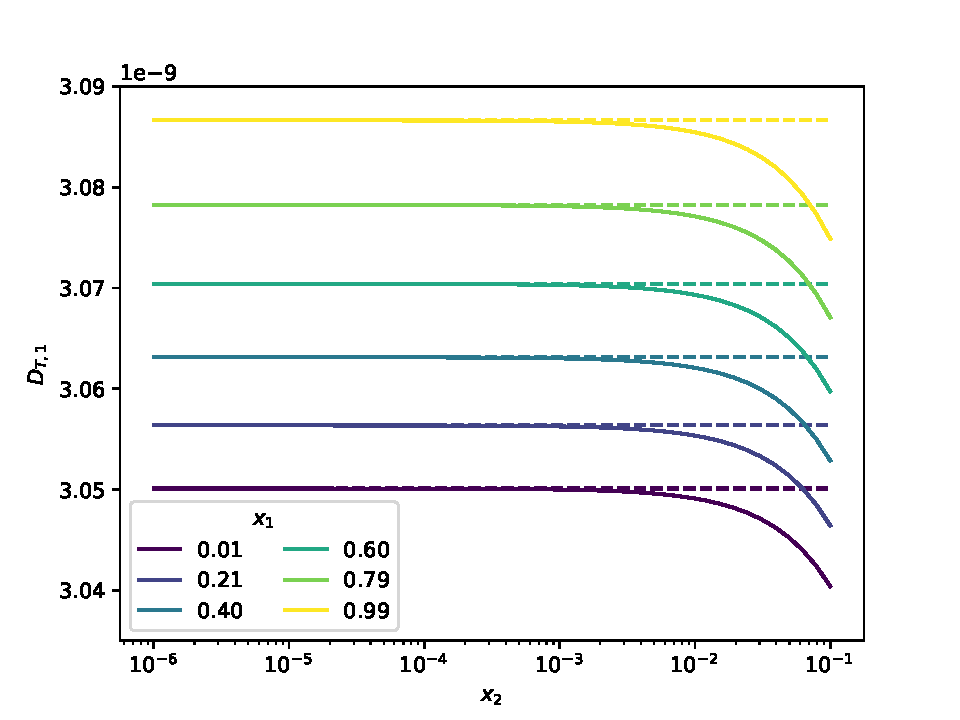
\includegraphics[width=.6\textwidth]{ternary_DT.pdf}
    \caption{The thermal diffusion coefficient $D_{T,1}^{(z, t)}$ in the ternary mixture (1, 2, 3) (solid lines), and the thermal diffusion coefficient $D_{T,1}^{z, b3}$ in the binary mixture (1, 3) (dashed lines), at different mole fractions of species 1 (colors). $x_1$ indicates the mole fraction of species 1 in the binary, i.e. $x_1 = n_1 / (n_1 + n_3)$, such that the composition of the ternary is $\Vec{x}_t = (x_1(1 - x_2), x_2, (1 - x_1)(1 - x_2))$.}
    \label{fig:ternary_DT}
\end{figure}

As seen immediately from Fig. \ref{fig:ternary_DT}, the ternary coefficient (solid lines) approaches the expected binary coefficient as $x_2 \to 0$. Note also the logarithmic scale, and that even at mole fractions of species 2 as small as $x_2 = 10^{-2}$, there is an appreciable difference in $D_{T,1}$ in the ternary compared to the corresponding binary. As seen more clearly in Fig. \ref{fig:ternary_DT_large}, the effect of increasing $x_2$ on $D_{T,1}$ is largest when $x_1$ is large. This could indicate that, contrary to intuition, if one wishes to model a ternary system with $x_1 > x_2 \gg x_3$ as a binary, neglecting the presence of species 3, a better estimate for thermal diffusion is obtained by taking species 2 as the independent species.

Explicitly: For a ternary system consisting of a trace component in air, the best estimate for thermal diffusion appears to be obtained if one models this as a binary mixture of nitrogen with the tracer \textit{taking the tracer to be the independent species}.

\begin{figure}[htb]
    \centering
    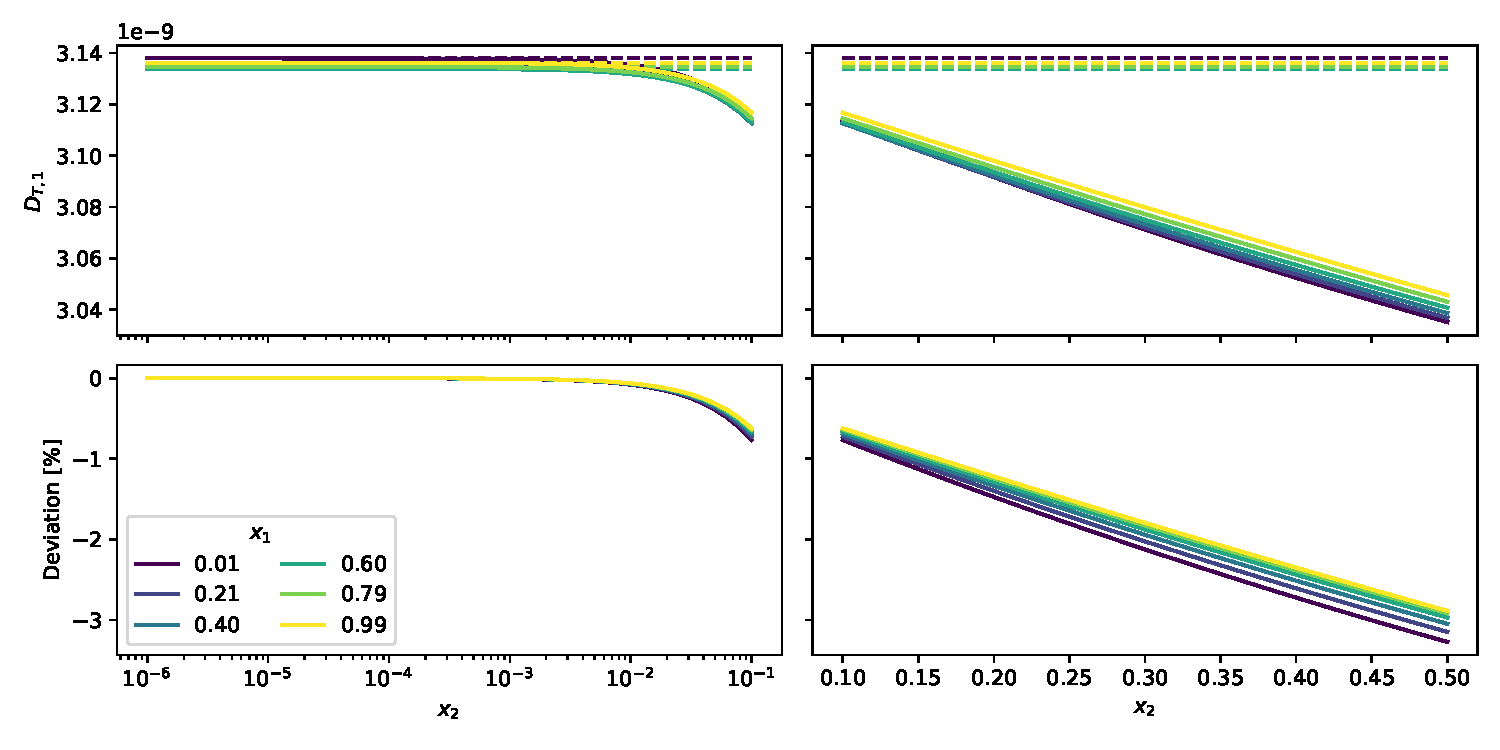
\includegraphics[width=.85\textwidth]{ternary_DT_large.pdf}
    \caption{The same thermal diffusion coefficients as in Fig. \ref{fig:ternary_DT}, with deviations and for a larger composition span.}
    \label{fig:ternary_DT_large}
\end{figure}